\section{Week-12 - 11.05.2026 - The 1-Dimensional Heat Equation }

\textbf{Last time:} We began studying the 1-dimensional heat equation.

\begin{center}
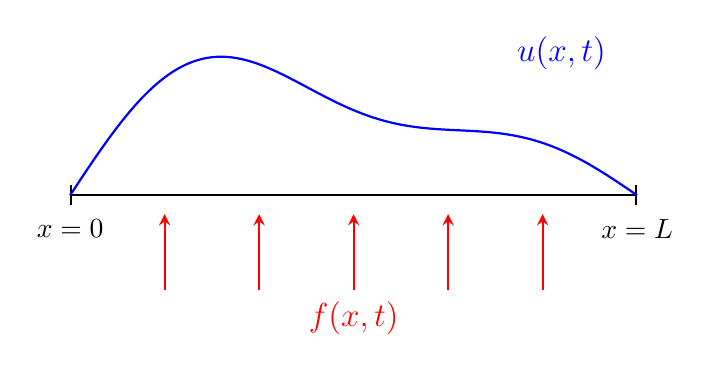
\begin{tikzpicture}[scale=1.2, thick]
    % X-axis
    \draw[|-|] (0,0) node[below=5pt]{$x=0$} -- (6,0) node[below=5pt]{$x=L$};
    
    % Function curve mathematically strictly zero at boundaries using a sine series
    \draw[blue, thick, smooth] plot[domain=0:6, samples=100] (\x, {1.2*sin(\x/6*180) + 0.4*sin(\x/6*360) + 0.3*sin(\x/6*540)});
    \node[blue] at (5.2, 1.5) {\large $u(x,t)$};
    
    % Force arrows
    \foreach \x in {1, 2, 3, 4, 5} {
        \draw[red, -stealth, thick] (\x, -1) -- (\x, -0.2);
    }
    \node[red] at (3, -1.3) {\large $f(x,t)$};
\end{tikzpicture}
\end{center}

\begin{definition}[Initial-Boundary Value Problem for the Heat Equation]
The problem is defined for $t > 0$ and $0 < x < L$ as:
\begin{align*}
    \frac{\partial u}{\partial t} - \frac{\partial^2 u}{\partial x^2} &= f \\[1ex]
    u|_{t=0} &= u_0 \quad \text{(initial condition)} \\[1ex]
    u|_{x=0} &= 0, \quad u|_{x=L} = 0 \quad \text{(boundary conditions)}
\end{align*}
\end{definition}

\textbf{Overview of the method:}
\begin{itemize}
    \item Decompose the heat equation into Fourier modes (in $x$).
    \item The PDE becomes an ODE (in time) for the Fourier coefficients. Solve it.
    \item Find a formula for the solution by summing the mode solutions.
\end{itemize}

\begin{theorem}[Uniqueness]
The initial value problem for the heat equation has a unique solution.
\end{theorem}

\begin{proofbox}
If $u_1$ and $u_2$ are two solutions, then their difference $v = u_1 - u_2$ solves the homogeneous problem:
\begin{align*}
    \frac{\partial v}{\partial t} - \frac{\partial^2 v}{\partial x^2} &= 0 \quad \text{for } t > 0, \ 0 < x < L \\
    v|_{t=0} &= 0 \\
    v|_{x=0} &= 0 = v|_{x=L}
\end{align*}
Consider the "energy" or $L^2$ norm of $v$:
\begin{equation*}
    \frac{\dd}{\dd t} \left( \int_0^L v^2(x,t) \, \dd x \right) = \int_0^L 2v \cdot \frac{\partial v}{\partial t} \, \dd x
\end{equation*}
Using the PDE $\frac{\partial v}{\partial t} = \frac{\partial^2 v}{\partial x^2}$, we substitute this in:
\begin{equation*}
    = 2 \int_0^L v \cdot \frac{\partial^2 v}{\partial x^2} \, \dd x
\end{equation*}
Integrating by parts:
\begin{equation*}
    = 2 \left( \left[ v \cdot \frac{\partial v}{\partial x} \right]_{x=0}^{x=L} - \int_0^L \left(\frac{\partial v}{\partial x}\right)^2 \dd x \right)
\end{equation*}
Since $v|_{x=0} = 0 = v|_{x=L}$, the boundary term evaluates to zero. Therefore,
\begin{equation*}
    = -2 \int_0^L \left(\frac{\partial v}{\partial x}\right)^2 \dd x \le 0
\end{equation*}
This implies that $\int_0^L v^2(t,x) \, \dd x$ is a decreasing function of $t$. Given the initial condition $v|_{t=0} = 0$, we have:
\begin{equation*}
    \int_0^L v^2(t,x) \, \dd x \le \int_0^L v^2(0,x) \, \dd x = 0
\end{equation*}
Since the integral of a non-negative function is strictly zero, we must have $v(t,x) = 0$ for all $t \ge 0$ and $0 \le x \le L$. Thus, $u_1 = u_2$.
\end{proofbox}

\begin{remark}[Implication of Uniqueness]
In view of uniqueness: If we can find a solution \textit{in any way}, then that is \textbf{the} unique solution.
\end{remark}

\subsection{Decomposing into Fourier Modes}

It helps to do the following trick: since we want $u|_{x=0} = 0$ and $u|_{x=L} = 0$, we extend $u(t,x)$ in $x$ to a $2L$-periodic function on $\R$ which is \textbf{odd}.

\begin{center}
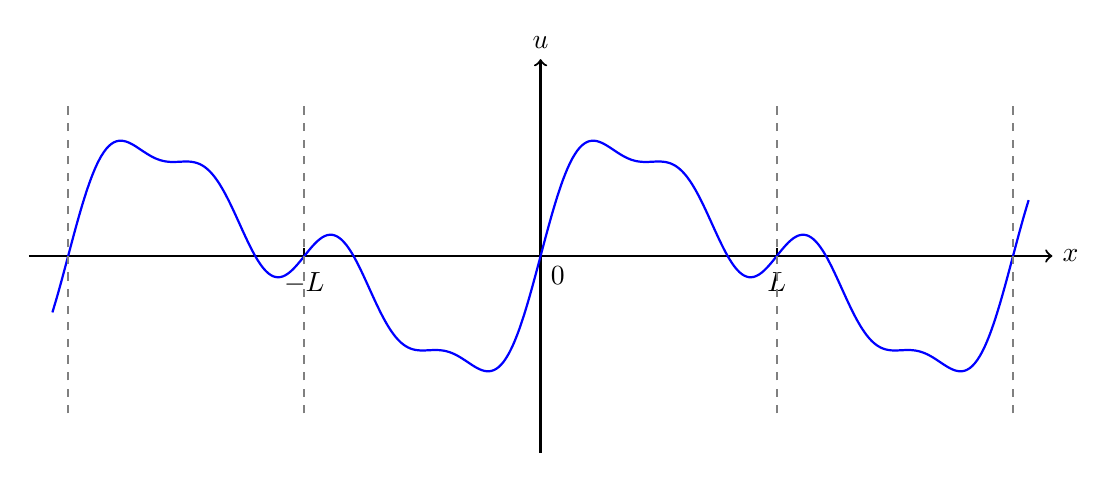
\begin{tikzpicture}[scale=1, thick]
    % Axes
    \draw[->] (-6.5,0) -- (6.5,0) node[right] {$x$};
    \draw[->] (0,-2.5) -- (0,2.5) node[above] {$u$};
    
    % Ticks
    \draw (-3,-0.1) -- (-3,0.1) node[below=5pt] {$-L$};
    \draw (3,-0.1) -- (3,0.1) node[below=5pt] {$L$};
    \node[below right] at (0,0) {$0$};

    % The odd, 2L-periodic function
    % Using a sum of sines ensures perfect mathematical oddness and periodicity
    \draw[blue, thick, smooth] plot[domain=-6.2:6.2, samples=200]
        (\x, {1.2*sin(\x/3*180) + 0.6*sin(\x/3*360) + 0.3*sin(\x/3*720)});

    % Adding dashed vertical lines to emphasize fundamental domain boundaries
    \draw[dashed, gray] (-3,-2) -- (-3,2);
    \draw[dashed, gray] (3,-2) -- (3,2);
    \draw[dashed, gray] (-6,-2) -- (-6,2);
    \draw[dashed, gray] (6,-2) -- (6,2);
\end{tikzpicture}
\end{center}

We do the same for $u_0$ and $f$. 
\textit{Note:} If $u$ is a $2L$-periodic and odd function which is continuous, then necessarily $u|_{x=0} = 0$ and $u|_{x=L} = 0$.

For the solution of the heat equation, it can be shown that if $f$ is piecewise continuous and the same is true for $u_0$, then for $t > 0$, $u(t,x)$ and $\frac{\partial u}{\partial x}(t,x)$ are continuous in $x$.

\textbf{Fourier series} (with respect to the $2L$-period):
Because of the odd extension, only sine terms appear.
\begin{align*}
    u(x,t) &= \sum_{n=1}^{\infty} b_n(t) \sin\left(\frac{\pi n}{L} x\right), \quad \text{where } b_n(t) = \frac{2}{L} \int_0^L u(x,t) \sin\left(\frac{\pi n}{L} x\right) \dd x \\
    u_0(x) &= \sum_{n=1}^{\infty} b_{0n} \sin\left(\frac{\pi n}{L} x\right) \\
    f(x,t) &= \sum_{n=1}^{\infty} f_n(t) \sin\left(\frac{\pi n}{L} x\right)
\end{align*}
Computing the derivatives:
\begin{align*}
    \frac{\partial u}{\partial x}(x,t) &= \sum_{n=1}^{\infty} b_n(t) \left(\frac{\pi n}{L}\right) \cos\left(\frac{\pi n}{L} x\right) \\
    \frac{\partial^2 u}{\partial x^2}(x,t) &= \sum_{n=1}^{\infty} b_n(t) \left(-\frac{\pi^2 n^2}{L^2}\right) \sin\left(\frac{\pi n}{L} x\right) \\
    \frac{\partial u}{\partial t}(x,t) &= \sum_{n=1}^{\infty} b_n'(t) \sin\left(\frac{\pi n}{L} x\right)
\end{align*}

Substituting these into the heat equation $\frac{\partial u}{\partial t} - \frac{\partial^2 u}{\partial x^2} = f$ gives:
\begin{equation*}
    \sum_{n=1}^{\infty} \left( b_n'(t) + \frac{\pi^2 n^2}{L^2} b_n(t) \right) \sin\left(\frac{\pi n}{L} x\right) = \sum_{n=1}^{\infty} f_n(t) \sin\left(\frac{\pi n}{L} x\right)
\end{equation*}

\begin{verification}[Mathematical Correction]
    In the original handwritten notes, a minus sign was written erroneously as $b_n'(t) - \frac{\pi^2 n^2}{L^2} b_n(t)$. This has been corrected to a \textbf{plus} sign here. This ensures mathematical accuracy because $\frac{\partial^2 u}{\partial x^2}$ already produces a negative term, so $-\frac{\partial^2 u}{\partial x^2}$ produces a strictly positive term.
\end{verification}

By matching the coefficients, for $n = 1, 2, 3, \dots$ and for $t > 0$, we get the ODE:
\begin{equation*}
    b_n'(t) + \frac{\pi^2 n^2}{L^2} b_n(t) = f_n(t)
\end{equation*}
With the initial conditions matching $u(x,0) = u_0(x)$, we have $b_n(0) = b_{0n}$.

The above is an initial value problem of the form:
\begin{equation*}
    \begin{cases}
    y' + ay = F \\
    y(0) = y_0
    \end{cases}
\end{equation*}
We have seen how to solve it (about 2 weeks ago) using the Laplace transform.

\begin{formula}[Solution for the Fourier Coefficients]
\begin{equation*}
    b_n(t) = b_{0n} e^{-\frac{\pi^2 n^2}{L^2}t} + \int_0^t e^{-\frac{\pi^2 n^2}{L^2}(t-s)} f_n(s) \, \dd s
\end{equation*}
So we have found $u$:
\begin{equation*}
    u(x,t) = \sum_{n=1}^{\infty} \left( b_{0n} e^{-\frac{\pi^2 n^2}{L^2}t} + \int_0^t e^{-\frac{\pi^2 n^2}{L^2}(t-s)} f_n(s) \, \dd s \right) \sin\left(\frac{\pi n}{L} x\right)
\end{equation*}
\end{formula}

\begin{remark}[Homogeneous Case]
If $f \equiv 0$, then $u(x,t) = \sum_{n=1}^{\infty} b_{0n} e^{-\frac{\pi^2 n^2}{L^2}t} \sin\left(\frac{\pi n}{L} x\right)$. 
This decays exponentially fast to 0 as $t \to +\infty$ (with an even faster decay in the higher modes).
\end{remark}

\begin{example}[Special Solution 1]
If $u_0 = 0$ and $f(x,t) = \sin\left(\frac{\pi x}{L}\right)$:
\begin{equation*}
    f_n(t) = 
    \begin{cases} 
    1, & n = 1 \\ 
    0, & n \ge 2 
    \end{cases}
\end{equation*}
This yields:
\begin{equation*}
    b_n(t) = 
    \begin{cases} 
    \frac{L^2}{\pi^2} \left(1 - e^{-\frac{\pi^2}{L^2}t}\right), & n = 1 \\ 
    0, & n \ge 2 
    \end{cases}
\end{equation*}
So the specific solution is:
\begin{equation*}
    u(x,t) = \frac{L^2}{\pi^2} \left(1 - e^{-\frac{\pi^2}{L^2}t}\right) \sin\left(\frac{\pi x}{L}\right)
\end{equation*}
\end{example}

\begin{remark}[Neumann Boundary Conditions]
If we wanted Neumann boundary conditions, namely $\frac{\partial u}{\partial x}\big|_{x=0} = 0 = \frac{\partial u}{\partial x}\big|_{x=L}$, we would extend $u$ as an \textbf{even} $2L$-periodic function. In that case, the series expansion uses cosines:
\begin{equation*}
    u(x,t) = \frac{a_0(t)}{2} + \sum_{n=1}^{\infty} a_n(t) \cos\left(\frac{\pi n}{L} x\right)
\end{equation*}
\end{remark}

\vspace{1em}
\hrule
\vspace{1em}

\subsection{The Wave Equation}

\textbf{Elastic cord:}

\begin{center}
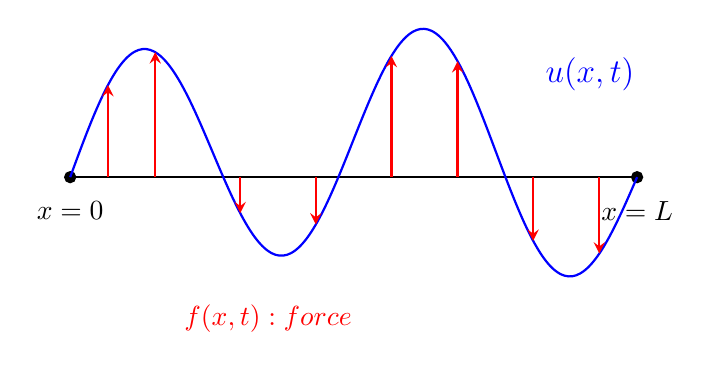
\begin{tikzpicture}[scale=1.2, thick]
    % X-axis
    \draw[-] (0,0) -- (6,0);
    \draw[fill=black] (0,0) circle (1.5pt) node[below=5pt]{$x=0$};
    \draw[fill=black] (6,0) circle (1.5pt) node[below=5pt]{$x=L$};

    % Wave curve mathematically enforced to cross axis multiple times
    \draw[blue, thick, smooth] plot[domain=0:6, samples=150]
        (\x, {1.2*sin(\x/6*720) + 0.4*sin(\x/6*180)});

    \node[blue, above] at (5.5, 0.8) {\large $u(x,t)$};

    % Force vectors (arrows calculated computationally to land exactly on the curve)
    \foreach \x in {0.4, 0.9, 1.8, 2.6, 3.4, 4.1, 4.9, 5.6} {
        \pgfmathsetmacro{\yval}{1.2*sin(\x/6*720) + 0.4*sin(\x/6*180)}
        \draw[red, -stealth, thick] (\x, 0) -- (\x, \yval);
    }

    \node[red, right] at (1.1, -1.5) {$f(x,t): \text{force}$};
\end{tikzpicture}
\end{center}

\begin{definition}[Initial-Boundary Value Problem for the Wave Equation]
Defined for $t > 0$ and $0 < x < L$:
\begin{align*}
    \frac{\partial^2 u}{\partial t^2} - c^2 \frac{\partial^2 u}{\partial x^2} &= f \\[1ex]
    u|_{t=0} &= u_0 \quad \text{(initial position)} \\
    \frac{\partial u}{\partial t}\bigg|_{t=0} &= u_1 \quad \text{(initial velocity)} \\[1ex]
    u|_{x=0} &= 0, \quad u|_{x=L} = 0 \quad \text{(Dirichlet boundary conditions: fixed endpoints)}
\end{align*}
Here, $c > 0$ is the speed of propagation.
\end{definition}

\begin{proposition}[Energy Conservation]
We define the energy $E[u](t)$ as the sum of kinetic and potential energy:
\begin{equation*}
    E[u](t) = \frac{1}{2} \int_0^L \underbrace{\left(\frac{\partial u}{\partial t}\right)^2}_{\text{Kinetic}} + \underbrace{c^2 \left(\frac{\partial u}{\partial x}\right)^2}_{\text{Potential}} \dd x
\end{equation*}
Then, the rate of change of energy equals the power exerted by the external force:
\begin{equation*}
    \frac{\dd}{\dd t} E[u](t) = \int_0^L \frac{\partial u}{\partial t}(x,t) f(x,t) \, \dd x
\end{equation*}
\end{proposition}

\begin{proofbox}
Differentiating the energy with respect to time:
\begin{equation*}
    \frac{\dd}{\dd t} E[u](t) = \frac{1}{2} \int_0^L 2\frac{\partial u}{\partial t} \cdot \frac{\partial^2 u}{\partial t^2} + 2c^2 \frac{\partial u}{\partial x} \cdot \frac{\partial^2 u}{\partial x \partial t} \, \dd x
\end{equation*}
Substitute $\frac{\partial^2 u}{\partial t^2} = c^2 \frac{\partial^2 u}{\partial x^2} + f$ into the first term:
\begin{equation*}
    = \int_0^L \frac{\partial u}{\partial t} \left( f + c^2 \frac{\partial^2 u}{\partial x^2} \right) + c^2 \frac{\partial u}{\partial x} \frac{\partial^2 u}{\partial x \partial t} \, \dd x
\end{equation*}
Separate the integral and apply integration by parts to $c^2 \frac{\partial u}{\partial t} \frac{\partial^2 u}{\partial x^2}$:
\begin{align*}
    = \int_0^L \frac{\partial u}{\partial t} f \, \dd x &+ \left[ c^2 \frac{\partial u}{\partial t} \frac{\partial u}{\partial x} \right]_{x=0}^{x=L} \\
    &- \int_0^L c^2 \frac{\partial^2 u}{\partial t \partial x} \frac{\partial u}{\partial x} \, \dd x + \int_0^L c^2 \frac{\partial u}{\partial x} \frac{\partial^2 u}{\partial x \partial t} \, \dd x
\end{align*}
The last two integrals perfectly cancel each other out. Since $u(0,t) = 0 = u(L,t)$, their time derivatives also vanish, $\frac{\partial u}{\partial t}(0,t) = 0 = \frac{\partial u}{\partial t}(L,t)$. Therefore, the boundary term vanishes.
\begin{equation*}
    \frac{\dd}{\dd t} E[u](t) = \int_0^L \frac{\partial u}{\partial t}(x,t) \cdot f(x,t) \, \dd x
\end{equation*}
\end{proofbox}

\begin{theorem}[Uniqueness]
The conservation of energy implies the uniqueness of solutions for the wave equation.
\end{theorem}
\begin{proofbox}
If $u_1$ and $u_2$ are two solutions, their difference $v = u_1 - u_2$ solves the homogeneous wave equation:
\begin{align*}
    \frac{\partial^2 v}{\partial t^2} - c^2 \frac{\partial^2 v}{\partial x^2} &= 0 \\
    v|_{t=0} &= 0 \\
    \frac{\partial v}{\partial t}\bigg|_{t=0} &= 0 \\
    v|_{x=0} &= 0 = v|_{x=L}
\end{align*}
Conservation of energy for $v$ (since $f=0$) implies $\frac{\dd}{\dd t} E[v](t) = 0$.
Thus, for all $t \ge 0$, $E[v](t) = E[v](0)$.
But $v|_{t=0} = 0$ and $\frac{\partial v}{\partial t}|_{t=0} = 0$ both vanish, so $E[v](0) = 0$.
So $E[v](t) = 0$.
Since $E[v](t) = \frac{1}{2} \int_0^L \left( \left(\frac{\partial v}{\partial t}\right)^2 + c^2 \left(\frac{\partial v}{\partial x}\right)^2 \right) \dd x = 0$, and the integrand is strictly non-negative, we infer that:
\begin{equation*}
    \frac{\partial v}{\partial t} = 0 \quad \text{and} \quad \frac{\partial v}{\partial x} = 0 \quad \forall t, x
\end{equation*}
Hence $v = \text{const}$. Since $v|_{t=0} = 0$, it follows that $v = 0 \implies u_1 = u_2$.
\end{proofbox}

\subsubsection{Construction of the Solution for the Wave Equation}

We extend $u(x,t)$, $f(x,t)$, $u_0(x)$, $u_1(x)$ as odd, $2L$-periodic functions of $x \in \R$.
The Fourier series then only contains sine terms:
\begin{align*}
    u(x,t) &= \sum_{n=1}^{\infty} b_n(t) \sin\left(\frac{\pi n}{L} x\right) \\
    u_0(x) &= \sum_{n=1}^{\infty} b_{0n} \sin\left(\frac{\pi n}{L} x\right) \\
    u_1(x) &= \sum_{n=1}^{\infty} b_{1n} \sin\left(\frac{\pi n}{L} x\right) \\
    f(x,t) &= \sum_{n=1}^{\infty} f_n(t) \sin\left(\frac{\pi n}{L} x\right)
\end{align*}

Differentiating yields:
\begin{align*}
    \frac{\partial^2 u}{\partial t^2}(x,t) &= \sum_{n=1}^{\infty} b_n''(t) \sin\left(\frac{\pi n}{L} x\right) \\
    \frac{\partial^2 u}{\partial x^2}(x,t) &= \sum_{n=1}^{\infty} b_n(t) \left(-\frac{\pi^2 n^2}{L^2}\right) \sin\left(\frac{\pi n}{L} x\right)
\end{align*}

Substituting into $\frac{\partial^2 u}{\partial t^2} - c^2 \frac{\partial^2 u}{\partial x^2} = f$ gives:
\begin{equation*}
    \sum_{n=1}^{\infty} \left( b_n''(t) + c^2 \frac{\pi^2 n^2}{L^2} b_n(t) \right) \sin\left(\frac{\pi n}{L} x\right) = \sum_{n=1}^{\infty} f_n(t) \sin\left(\frac{\pi n}{L} x\right)
\end{equation*}

This generates a system of ODEs for the coefficients:
\begin{equation*}
    \begin{cases}
    b_n''(t) + c^2 \frac{\pi^2 n^2}{L^2} b_n(t) = f_n(t) \\
    b_n(0) = b_{0n} \\
    b_n'(0) = b_{1n}
    \end{cases}
\end{equation*}

We can solve this using the Laplace transform:
\begin{equation*}
    z^2 \Lap[b_n](z) - z b_n(0) - b_n'(0) + \frac{c^2 \pi^2 n^2}{L^2} \Lap[b_n](z) = \Lap[f_n](z)
\end{equation*}
\begin{equation*}
    \implies \Lap[b_n](z) = \frac{\Lap[f_n](z) + z \cdot b_{0n} + b_{1n}}{z^2 + \frac{c^2 \pi^2 n^2}{L^2}}
\end{equation*}

Taking the inverse Laplace transform for $n = 1, 2, 3, \dots$:
\begin{equation*}
    b_n(t) = b_{0n} \cos\left(\frac{c\pi n}{L}t\right) + \frac{b_{1n}}{c\frac{\pi n}{L}} \sin\left(\frac{c\pi n}{L}t\right) + \int_0^t \frac{1}{c\frac{\pi n}{L}} \sin\left(\frac{c\pi n}{L}(t-s)\right) f_n(s) \, \dd s
\end{equation*}

\begin{example}[Special Cases for the Wave Equation]
\textbf{Case 1:} If $f \equiv 0$, $u_0 = \sin\left(\frac{\pi x}{L}\right)$, and $u_1 = 0$:
\begin{align*}
    f_n(t) &= 0 \\
    b_{0n} &= 
    \begin{cases}
    1, & n = 1 \\
    0, & n \ge 2
    \end{cases} \\
    b_{1n} &= 0
\end{align*}
This implies $b_n(t) = \cos\left(\frac{c\pi}{L}t\right)$ for $n=1$, and $0$ otherwise. The final solution is:
\begin{equation*}
    u(x,t) = \cos\left(\frac{c\pi}{L}t\right) \sin\left(\frac{\pi x}{L}\right)
\end{equation*}

\textbf{Case 2:} If $u_0 = 0$, $u_1 = 0$, and $f(x,t) = \sin\left(\frac{\pi x}{L}\right)$:
\begin{align*}
    b_{0n} &= 0 \\
    b_{1n} &= 0 \\
    f_n(t) &= 
    \begin{cases}
    1, & n = 1 \\
    0, & n \ge 2
    \end{cases}
\end{align*}
By explicitly evaluating the integral for $n=1$, we get:
\begin{equation*}
    b_1(t) = \frac{1 - \cos\left(\frac{c\pi}{L}t\right)}{\left(c\frac{\pi}{L}\right)^2}
\end{equation*}
\begin{verification}[Mathematical Correction]
    The handwritten notes omitted the square in the denominator: $c\frac{\pi}{L}$. Standard integration of $\int \frac{1}{\omega} \sin(\omega(t-s)) \, ds$ yields $\frac{1-\cos(\omega t)}{\omega^2}$. Hence it is explicitly corrected here to $\left(c\frac{\pi}{L}\right)^2$.
\end{verification}
The specific solution is:
\begin{equation*}
    u(x,t) = \frac{1 - \cos\left(\frac{c\pi}{L}t\right)}{\left(c\frac{\pi}{L}\right)^2} \sin\left(\frac{\pi x}{L}\right)
\end{equation*}
\end{example}

\vspace{1em}
\hrule
\vspace{1em}

\subsection{Generalizing the Method}

\begin{remark}[Extensions of the Fourier Method]
The above method applies to more general initial-boundary value problems ($x \in [0,L], t \ge 0$) for linear PDEs, subject to the following principles:

\begin{enumerate}
    \item \textbf{Constant Coefficients:} We typically need the coefficients of the spatial operator in the equation to be constant with respect to $x$.
    For example, if we try the same approach for:
    \begin{equation*}
        \frac{\partial^2 u}{\partial t^2} - c^2(t) \frac{\partial^2 u}{\partial x^2} = f
    \end{equation*}
    It yields the ODE:
    \begin{equation*}
        b_n''(t) + c^2(t) \frac{\pi^2 n^2}{L^2} b_n(t) = f_n(t)
    \end{equation*}
    In principle, if $c(t)$ is known explicitly, the above ODE can be solved, but it is much more complicated than the case of a constant $c$.
    
    \item \textbf{General Boundary Conditions:} One can also address more general boundary conditions, e.g., periodic boundary conditions:
    \begin{align*}
        u(0,t) &= u(L,t) \\
        \frac{\partial u}{\partial x}(0,t) &= \frac{\partial u}{\partial x}(L,t)
    \end{align*}
    In this case, decomposing relies on the full Fourier series:
    \begin{equation*}
        u(x,t) = \frac{a_0(t)}{2} + \sum_{n=1}^{\infty} \left( a_n(t) \cos\left(\frac{2\pi n}{L}x\right) + b_n(t) \sin\left(\frac{2\pi n}{L}x\right) \right)
    \end{equation*}
    And we solve coupled ODEs for both $a_n(t)$ and $b_n(t)$.
    
    \item \textbf{Inhomogeneous Boundary Conditions:} (Covered in exercise sets).
    
    \item \textbf{General Linear Operators:} Solving initial-boundary value problems of the form:
    \begin{align*}
        \frac{\partial u}{\partial t} + P u &= 0 \\
        u|_{t=0} &= u_0 \\
        u|_{x=0} &= 0, \quad u|_{x=L} = 0
    \end{align*}
    Where $P$ is a linear differential operator:
    \begin{equation*}
        P = c_k(x) \frac{\partial^k}{\partial x^k} + \dots + c_1(x) \frac{\partial}{\partial x} + c_0(x)
    \end{equation*}
    This requires decomposing $u(x,t)$ into a series \textit{not necessarily trigonometric}, but rather with respect to a basis of \textbf{"eigenfunctions"} of $P$ (with Dirichlet boundary conditions), known as a \textbf{Sturm-Liouville problem}.
    
    In this class, we will not deal with this more general case; we will strictly consider problems where the trigonometric series is the appropriate expansion.
\end{enumerate}
\end{remark}

\subsection{Fourier Transform and PDEs}

While on $x \in [0,L]$ we utilize the Fourier series decomposition, on the whole real line $x \in \R$, we shift to the \textbf{Fourier transform} in $x$.

\begin{recall}[Fourier Transform on $\R$]
For an absolutely integrable function $f: \R \to \C$ (provided $\int_{-\infty}^{+\infty} |f(x)| \, \dd x < +\infty$), the Fourier transform is defined as:
\begin{equation*}
    \mathcal{F}[f](\xi) = \hat{f}(\xi) = \frac{1}{\sqrt{2\pi}} \int_{-\infty}^{+\infty} e^{-i\xi x} f(x) \, \dd x
\end{equation*}
\end{recall}